\chapter{Classification methods }
In previous chapter, we introduce a method to remove the unexpected object. In this chapter, we will propose a method to obtain the features what we are interested in and the method to detect the landmarks on the insect. This method was proposed by Palaniswamy$^{\cite{palaniswamy2010automatic}}$. The processes can be discuss in follow steps:
\begin{enumerate}
\item Extracting the features:
\item Constructing and comparing the pairwise geometric histogram
\item Estimating the pose by the probabilistic Hough transform
\item Detecting the landmarks by template matching
\end{enumerate}
\section{Preprocessing image and feature extraction}
To obtain the good result, before extracting the features in the image, we need to pre-process the image with a appropriate technique to reduce the noise as well as enhance the features that we care. 
Feature extraction is a process extracting interested features from digital image. The expect result in this result is list of approximate lines which use to construct the pairwise geometric histogram. \\[0.2cm]
The process mainly separate into two stages: Firstly, we pre-process image. In this stage, we reduce the noise in image by finding a threshold value and apply the thresholding technique to obtain the interested features. Secondly, we extract the features based on the edge segmentation. By applying the appropriate technique to obtain the step edges and broken the edges into approximate lines.
\subsection{Preprocess image}
In this application, we use the thresholding technique to pre-process the image. In thresholding technique, with a threshold value ``t", we can decrease the noise and obtain the interested features. The threshold value can be defined by the histogram analysis.\\[0.2cm]
Based on the histogram of the original image, we compute the mean and median of this histogram. With the histogram obtained, we split it into two parts: the first part begin from the bin 0 to the limit value (the limit value is smallest value between mean and median); the second part, starting from the limit value to the end of histogram. For each part, we find the maximum, minimum value and calculating the mean of it. The value ``t" obtained by the mean of two mean values in two parts of histogram.\\
With the threshold value ``t", we apply the threshold technique to pre-process image in the CV\_THRESH\_BINARY mode (keep the pixel has value greater than threshold value).\\
\IncMargin{1em}
\begin{algorithm}[H]
\Indm 
\KwData{inputImage: the input image}
\KwResult{outputImage: the image after processing}
\Indp
Convert the input image into gray scale image\;
Calculate the histogram on gray scale image and store the result in $histogram$ variable \;
Compute the $mean$ value and $median$ value of histogram\;
$limit \leftarrow (mean > median$ ? $median : mean)$\;
$limitSub \leftarrow ((limit >= 120)$ ? $(limit - 25) : (limit - 5))$\;
Declare some variables: $int$ $imax \leftarrow -1, max \leftarrow -1$\;
\For{$i \leftarrow$ 0 to $limitSub$}{
	\If{$histogram[i]$ $>$ $max$}{
		$max$ = $histogram[i]$\;
		$imax$ = $i$\;
	}
}
Declare some variables: $int$ $imin \leftarrow -1, min \leftarrow max$\;
\For{$k \leftarrow$ imax to $limit$}{
	\If{$histogram[k]$ $<$ $min$}{
		$min$ = $histogram[k]$\;
		$imin$ = $k$\;
	}
}
Declare some variables: $int$ $max2 \leftarrow -1, imax2 \leftarrow -1$\;
\For{$j \leftarrow limit $ to $end\_of\_histogram$}{
	\If{$histogram[j]$ $>$ $max2$}{
		$max2$ = $histogram[j]$\;
		$imax2$ = $j$\;
	} 
}
$middle1 \leftarrow (imax1 + imin)/2$ \;
$middle2 \leftarrow (imax2 + imin)/2$ \;
$middle \leftarrow (middle1 + middle2)/2$ \;
Apply the threshold with threshold value is $middle$\;
\caption{Algorithm to preprocess image}
\end{algorithm}\DecMargin{1em}
\subsection{Feature extraction}
After apply the threshold to pre-process image, we apply the Canny algorithm to detect the step edges, which incorporates non-maximal suppression and hysteresis thresholding. In Canny, the importance parameters are two threshold values and aperture size for the Sobel operator, it decides the pixels kept. The threshold value used in Canny algorithm also the value used in the previous step, and the ratio between lower threshold and upper threshold is 1.5 : 3 (follows the article \cite{palaniswamy2010automatic}). In implementation, the Canny operation used from OpenCV library\footnote{http://docs.opencv.org/modules/imgproc/doc/feature\_detection.html\#canny}, and the parameters need to put into Canny are:
\begin{itemize}
\item source: the input image (in grayscale mode)
\item destination: the output image
\item low\_thresh: the first (lower) threshold value
\item hight\_thresh: the second (upper) threshold value
\item kernel\_size: size of kernel, aperture for the Sobel operator
\end{itemize}
The Canny algorithm is not aware of actual edges, the edge detecting was based on the Sobel operator, extracted with non-maximal suppression. So, to obtain the expect result, we  need to apply another technique to obtain the step edges. The \textbf{findContours} was chosen for this aim, the result is a vector of the edges, and each edge was presented by a vector of the points. Like the Canny, the \textbf{findContours} also used from OpenCV library \footnote{http://docs.opencv.org/modules/imgproc/doc/structural\_analysis\_and\_shape\_descriptors.html\#findcontours} and the parameters used in this operation as follows:
\begin{itemize}
\item source: the binary input image
\item contours: the output. Each contours is stored in a vector of points.
\item hierarchy: optional output vector, containing information about the image topology.
\item mode: contours retrieve mode
\item method: contours approximation method
\item offset: optional offset by which every contour point is shifted.
\end{itemize}
\subsection{Edge segmentation}
The geometric relation can not constructed from the edges, it always construct from the relation of basic geometric objects, such as the lines.  In fact, any arbitrary edge can be represented by a set approximate lines. Instead of representing an edge, we can represent a set of approximate lines of it. This way also useful when we want presentation the edges or describe the relation between it. With the set of step edges was obtained from find contours (the image structure). In this step, we will segment it to approximated lines. The method to segment the edges is a recursive algorithm$^{\cite{riocreux1994analysis}}$ but it have some change in the ``stop condition" of algorithm to easy process, as follows:
\begin{itemize}
\item Establish a line \textit{``l"} between two endpoints of edge.
\item For each point on edge, we compute the perpendicular distance from it to the line l and keep the point which has the maximum perpendicular distance.
\item If the maximum perpendicular distance from a point on edge to the line \textit{l} is greater than $\alpha$, then the edge is split at this point. The value chosen for $\alpha$ in the program is 3 ($\alpha = 3$).
\item Reprocess both parts which was obtained from step 3.
\item The algorithm continues until all edges fragments are represented.
\end{itemize}
The algorithm is presented as follows:\\
\IncMargin{1em}
\begin{algorithm}[H]
\Indm 
\KwData{listPoints: list of points which presented the edge}
\KwResult{Queue of ``step" points on the edge}
\Indp
Declare the first endpoint: $p0 \leftarrow listPoints[0]$\;
Declare the second endpoint: $pend \leftarrow listPoints[size - 1]$, \textit{size} is the size of \textit{listPoints}\;
Set up a straight line between the two endpoints $p0, pend$ (line $d$)\;
Initialization the max value: $maxDistance  \leftarrow 0 $\;
Declare a ``split point": $imax \leftarrow 0$ \; 
Declare a variable: $distance \leftarrow 0$\;

\For{ point $p$ in $listPoints$}{
	$distance \leftarrow$ from $p$ to line $d$\;
	\If{distance $>$ max\_distance}{
		$maxDistance$ $\leftarrow$ $distance$\;
		$imax$ $\leftarrow$ position of $p$\;
	}
}
\If{$maxDistance$ $>$ 3 }{
	split the list of points at $imax$ and put into 2 parts $(part1, part2)$\;
	Pre-process on $part1$\;	
	Pre-process on $part2$\;
}
\If {$p0$ does not exist in result queue}{
	push $p0$ into queue\;\tcp{queue is a variable of class}
}
\If {$pend$ does not exist in result queue}{
	push $pend$ into queue\;\tcp{queue is a variable of class}
}
\caption{Algorithm to segment an edge}
\end{algorithm}\DecMargin{1em}
\section{Pairwise geometric histogram}
Pairwise geometric histogram(PGH) is used to encode the relative information between a line and a set of lines in an object. Therefore, an object can represented by a set of PGH. From the set of PGH, we can reconstructed the object or compare with another object. In this section, we will mention the constructing a PGH for an object based on the geometrical relationship and compute the similar distance between two objects.

\subsection{Local pairwise geometric histogram}
The PGH is constructed on the geometric features between lines relative. The geometric features are characteristic which can describe the geometric shape such as angle, the length of line, perpendicular between two lines,.... For the shape representation, the relative angle and perpendicular distance is geometrical features useful. \\
The Local PGH presented the relationship between a reference line with another lines. The proceed to construct the PGH between two lines was described in below:
\begin{itemize}
\item Choose the reference line (other lines called object lines)
\item Compute the angle between reference line and the object lines
\item Calculate the perpendicular distance from two endpoints of object lines to the reference line (assigned dmin and dmax).
\item Recording the perpendicular distance and angle relative between reference line and the object lines into the two dimensional histogram.
\end{itemize}
Example \footnote{Images extract from the article \cite{palaniswamy2010automatic}}:\\
\begin{figure}[h!]
\centering
\subfloat[The geometric relationship between two lines]{\label{fig:example_1}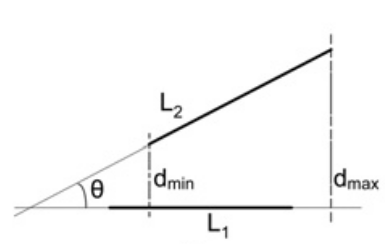
\includegraphics[width=0.4\textwidth]{./images/PGH_geo}}~~
\subfloat[The pairwise geometric histogram ]{\label{fig:example_2}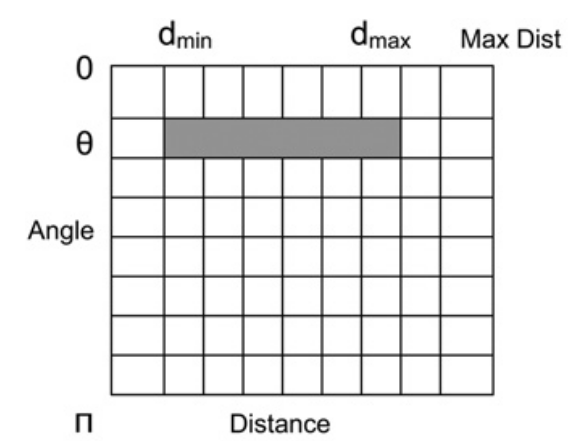
\includegraphics[width=0.4\textwidth]{./images/PGH}}
\caption{The geometric features and the PGH}
\label{fig:figure_31}
\end{figure}
\\[0.3cm]The frequency of the geometric features is recorded as a two dimensional histogram with an angle axis (0 - $\pi$) and distance axis (range of perpendicular distance, $d_{max}$ is the maximum distance on all distance of two arbitrary lines). The entries on PGH describe the geometric relationship between the reference line and the object lines. The blurring of entry along the axis regarding the true position and orientation of each object lines for reference line. Following the accuracy, we can indicate the size of histogram and normalize the value to match with size of histogram.
\subsection{Global pairwise histogram}
Based on the constructor of a line in object. The object encoded by recording PGH for all lines within object. If the object is defined by n lines, the full shape representation will composed of n pairwise geometric histograms.\\
This method still good when we apply some variants on the image, such as translate or rotate the image because the angle and perpendicular distance between a pair of lines is invariant.
\subsection{Histogram matching}
``The histogram matching enables robust classification of shape features by finding similarity between the scene and reference model"$^{\cite{palaniswamy2010automatic}}$. The similar between two models can obtain via the similar distance, which was computed by comparing their probability distribution on geometric histogram. In program, each image was represented by a comprises of many geometric histograms and using the Bhattacharyya metric to determine the similar distance between two models $^{\cite{palaniswamy2010automatic}}$. In general, we have normalize the histograms before comparing. The form of Bhattacharryya metric used to compute the degree of 2 model:
\begin{center}
\begin{equation} \label{eq:1}
d_{Bhattacharyya} (H_{i}H_{j}) = \sum\limits_{\theta}^{\pi}\sum\limits_{d}^{d_{max}}\sqrt{H_{i}(\theta,d)H_{j}(\theta,d)}
\end{equation}
\end{center}
The significance of parameters in the formula \ref{eq:1}, as follows:
\begin{itemize}
\item $\theta$: angle value, range of $\theta$ in angle axis from 0 to $\pi$.
\item $d$: the perpendicular distance, range of d in perpendicular distance from 0 to the maximum distance of arbitrary lines of shape.
\item $H_{i}(\theta,d)$ is an entry at row $\theta$ and column d in histogram of image \textit{i}
\item $H_{j}(\theta,d)$ is an entry at row $\theta$ and column d in histogram of image \textit{j}
\end{itemize}
By the default, the range of angle axis from 0 to 180 degree (correspondence with 180 degree). Based on the accuracy of program, we can increase the range of angle axis. This design allow increase the range of angle axis to several time with default value. Example, the table below show the result when calculating Bhattacharyya distance between image \textit{Md 028.JPG} and some images with difference accuracy:
\begin{center}
\begin{tabular}{|l|l|c|c|c|c|c|c|}
\hline
Reference image & Scene image & 180 & 2 * 180 & 4 * 180 & 6 * 180 \\ \hline
Md 028.JPG & Md 001.JPG & 0.977953 & 0.964167 & 0.93861 & 0.91471 \\ \hline
Md 028.JPG & Md 005.JPG & 0.96479 & 0.943657 & 0.906444 & 0.871756  \\ \hline
Md 028.JPG & Md 010.JPG & 0.976241 & 0.958061 & 0.925943 & 0.896445 \\ \hline
Md 028.JPG & Md 027.JPG & 0.980728 & 0.968233 & 0.945442 & 0.92485 \\ \hline
\end{tabular}
\end{center}
Besides the Bhattacharyya metric, we can also choose another metric to matching the histograms, such as: \textbf{Chi-squared} metric and \textbf{Intersection} metric. The forms was presented as below:\\
\textbf{Chi-squared metric:}
\begin{center}
\begin{equation}\label{eq:2}
d_{Chi-squared} (H_{i}H_{j}) = \frac{\sum\limits_{\theta}^{\pi}\sum\limits_{d}^{d_{max}}(\frac{(H_{i}(\theta,d) - H_{j}(\theta,d))^{2}}{(H_{i}(\theta,d) + H_{j}(\theta,d))})}{2}
\end{equation}
\end{center}
\textbf{Intersection metric}
\begin{center}
\begin{equation}\label{eq:3}
d_{Intersection} (H_{i}H_{j}) = \sum\limits_{\theta}^{\pi}\sum\limits_{d}^{d_{max}}min(H_{i}(\theta,d), H_{j}(\theta,d))
\end{equation}
\end{center}
The significance of parameters in equation (\ref{eq:2}) and (\ref{eq:3}) is similar with (\ref{eq:1}). For the Bhattacharyya and Intersection metric, the perfect match is 1 and the total mismatch is 0. The result is opposite to Chi-squared metric (0 for perfect match and 1 for total mismatch).\\[0.2cm]
Hence, depend on the purpose of comparison will choose a suitable comparing method. In this program, we want to try on three method to have a general view result when matching the histograms.
\subsection{Probabilistic Hough transform}
The probabilistic Hough transform (PHT) used to estimate the global shape. Based on a group of features within the scene, identifying the present of a model image in a scene image. The hypothesised location of the model in the scene is indicated based on the conditional probability that any pair scene lines agreement about a position in model.\\[0.3cm]
Estimating the global shape has two main stages. Firstly, training process begin by recording the perpendicular distance and the angle from a reference point to each pair of model lines. Secondly, predicting the pose of scene difference from the model, then we estimate the location of the landmarks. We create a Hough space to store value when exist a pair of scene lines match with the entry in training process. The peak in Hough space is assumed of the reference point of the model in the scene. From this reference point, we can estimate the reference landmarks of reference image on the scene.
The process to estimate the global pose is described as follows:
\begin{itemize}
\item Choose a arbitrary point in model as reference point
\item For each pair lines in model, calculating and recording the perpendicular distance and angle from the reference point to each line.
\item Create an two dimensional accumulator, one dimension for the angle and another for the perpendicular distance.
\item For each pair lines in scene, finding the entry correspond about position, orientation and scale. Increase the value at correlative cell in the accumulator (indicate by the angle and distance).
\item Compute the maximum value in accumulator.
\item Indicating the pair of scene lines and the entry with maximal value of accumulator.
\item Extending the perpendicular lines of the pair of scene lines at the appropriate position. The intersection of them is the location of reference point in the scene.
\end{itemize}
In the example below, we apply the PHT to estimate the landmarks of model in the scene. The image in figure \ref{fig:pht_1} as the model. In the model, the small red circle and large red circles are the reference point and the landmarks in model, respectively. The image in figure \ref{fig:pht_2} as scene. By applying the PHT, we can estimate the reference point (green circle) in the scene and the location of the landmarks (the yellow circles).
\begin{figure}[h!]
\centering
\subfloat[The model image]{\label{fig:pht_1}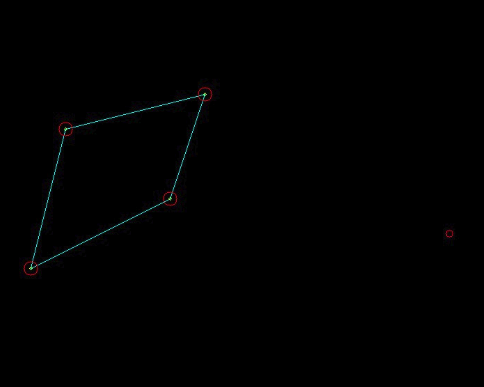
\includegraphics[width=0.35\textwidth]{./images/pht_1}}~~
\subfloat[The scene image ]{\label{fig:pht_2}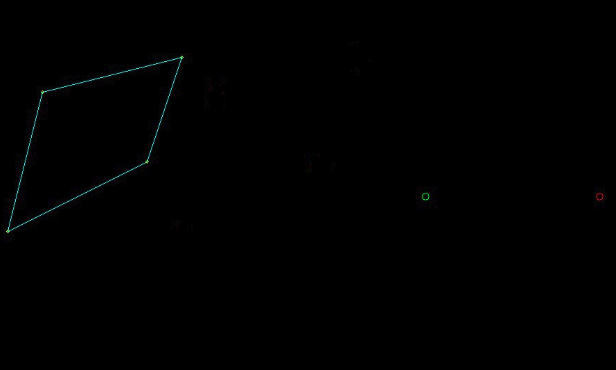
\includegraphics[width=0.35\textwidth]{./images/pht_2}}
\caption{The landmarks estimated by probabilistic Hough transform}
\label{fig:figure_31}
\end{figure}
\subsubsection{Training process}
In this step, recording the perpendicular distance and angle from each pair model lines to a reference point (called reference table). The reference point can be chosen at arbitrary position on model image. To save the time to process at the next step, we just consider the ``closet pair lines". In this application, the reference point chosen at the center of image and the closet pair lines are pair of lines have all three conditions: the length of each line greater than 60 pixels, the lines are not parallel and the distance between it less than 5 pixels. The algorithm to consider a pair closet lines and construct the reference table as follows:\\[0.2cm]
\begin{algorithm}[H]
\Indm 
\KwData{line1 (the first line), line2 (the second line)}
\KwResult{Two line closet or not (bool)}
\Indp
$distance1$ $\leftarrow$ distance from the first endpoint of $line1$ to $line2$\;
$distance2$ $\leftarrow$  distance from the second endpoint of $line1$ to $line2$\;
\If {$line1.length() > $ 60 and $line2.length() > $60  \\
		and $line1$ not parallel with $line2$\\
		and ($distance1$ $<=$ 5 or $ditance2$ $<=$ 5 )}{
	$return$ $true$\;
}
return $false$\;
\caption{Algorithm to consider the closet lines}
\end{algorithm}~\\[0.2cm]
\begin{algorithm}[H]
\Indm 
\KwData{lines (a list of lines), refPoint (the reference point)}
\KwResult{The reference table}
\Indp
Declare the reference table $refTable$ \;
\For{ line $i$ in $lines.size()$}{
	\For{line $j$ in $lines.size()$}{
		\If{i $!=$ j and $line(i)$ closet with $line(j)$}{
			Compute the angle and perpendicular distance from $line(i)$ to $refPoint$\;
			Compute the angle and perpendicular distance from $line(j)$ to $refPoint$\;
			Create an entry to store pair of lines and its information \;
			Add the entry into reference table \;
		}
	}
}
return reference table \;
\caption{Algorithm to construct the reference table}
\end{algorithm}~\\
\subsubsection{Estimating process}
The estimating process is duration estimate the reference landmarks on the scene image. Firstly, we need to find the reference point on scene image. Secondly, we estimate the reference landmarks on the scene image from the reference point.\\[0.2cm]
By finding a pair of scene lines agree with a pair of model lines, we can detect the position of the reference point on scene image. We create an accumulator to store each agreement between pair of scene lines and pair of model lines. For each pair of scene lines, we find its exist in the reference table and increase the value at correspondence position in accumulator. At the end, we can obtain the pair of scene lines and pair of model lines correspondence with the maximum value in accumulator. By extending the perpendicular lines of the pair of scene lines at the appropriate position, we can meet the reference point at the intersection of them.\\[0.2cm]
In this program, two pair lines called agreement if the angle difference between them less than one degree and the length scale less than two. Two algorithm followed describe the definition between two pair lines and finding the position of reference point in scene image.\\[0.2cm]
\begin{algorithm}[H]
\Indm 
\KwData{line1 (the first reference line), line2 (the second reference line), sline1 (the first scene line), sline2 (the second scene line)}
\KwResult{Two pair lines similar or not (boo)}
\Indp
$angle1$ $\leftarrow$ angle between $line1$ and $line2$\;
$angle2$ $\leftarrow$ angle between $sline1$ and $sline2$\;
\If{$abs(ange1$ - $angle2) < 1$ $and$ $abs(line1.length()/sline1.length()$ - $line2.length()/sline2.length()) < 2$}{
	return $true$\;
}
return $false$ \;
\caption{Algorithm to check the agreement between two pair lines}
\end{algorithm}~\\[0.2cm]
\begin{algorithm}[H]
\Indm 
\KwData{refTable (the reference table), slines (pair of scene lines)}
\KwResult{The entry in reference table}
\Indp
Declare the entry in reference table $entry$ \;
\For{ entry $et$ in $refTable$}{
	\If{agree between lines in entry and $slines$}{
		$entry$ $\leftarrow$ $et$\;
	}
}
return $entry$ \;
\caption{Algorithm to find the agreement of pair scene lines in model}
\end{algorithm}~\\[0.2cm]
\begin{algorithm}[H]
\Indm 
\KwData{lines (a list of scene lines), refTable (reference table)}
\KwResult{The reference table}
\Indp
Create an accumulator, $acc$\;
Declare the reference table $refTable$ \;
\For{ line $i$ in $lines.size()$}{
	\For{line $j$ in $lines.size()$}{
		\If{i $!=$ j and $line(i)$ closet with $line(j)$}{
			Find the agreement of pair scene lines in mode\;
			Increase the value in $acc$ with correspondence position\;
			Marked the maximum value, pair of scene lines and entry in reference table\;
		}
	}
}

Find the intersection ($intersect$) between two perpendicular lines with pair scene lines at appropriate position\;
\tcp{The appropriate position is correct with the distances in reference table.}
return $intersect$ \;
\caption{Algorithm to find the reference point in scene}
\end{algorithm}~\\[0.2cm]
By finding the reference point, the landmarks in scene image can be estimated by calculating the relative between the reference point and the reference landmarks. Besides, we also record the difference about rotation, orientation and scale between model image and scene image.
\subsection{Template matching}
Template matching is duration to refine the estimated landmarks on the scene image with an appropriate method.
\subsubsection{Cross-correlation}
Cross-correlation is a method of estimating the similarity between two signals. By computing the sum of product between 2 signals when sliding, and choose the maximal value. It is used for searching a short signal in a longer signal. In image processing, it used to detect the present of an object (template) in a large object (image). The equation of cross-correlation as follows (equation \ref{eq:cross-correlation}):
\begin{center}
\begin{equation}\label{eq:cross-correlation}
R_{ccorr}(x,y) = \sum\limits_{x',y'}[T(x'.y').I(x + x', y + y')]
\end{equation}
\end{center}
Where:
\begin{itemize}
\item T is template which use to slide and find the exist in other image.
\item I is image which we expect to find the template image
\item $(x', y')$ are coordinates in template where we get the value to compute.
\item $(x + x', y + y')$ are coordinates in image where we get the value to compute when template $T$ sliding.
\end{itemize}
By sliding the template on image by each pixel from left to right and top to down. At each position, we compute the $R_{ccorr}(x,y)$. The position have maximal $R_{ccorr}(x,y)$ is position that best similar of template in image.\\[0.2cm]
However, if we use the original image to compute and find the similarity, the brightness of template and image can change the conditions and the result. So, we can be normalize the image before apply the cross-correlation to reduce the effect of lighting difference between them. The normalization coefficient is:
\begin{center}
\begin{equation}\label{eq:normalizeCoff}
Z(x,y) = \sqrt{\sum\limits_{x',y'}T(x'.y')^{2}.\sum\limits_{x',y'}I(x + x', y + y')^{2}}
\end{equation}
\end{center}
The value of this method when we normalized computation as below:
\begin{center}
\begin{equation}\label{eq:cross-correlation}
R_{ccorr\_norm}(x,y) =\frac{R_{ccorr}(x,y)}{Z(x,y)} = \frac{\sum\limits_{x',y'}[T(x'.y').I(x + x', y + y')]}{\sqrt{\sum\limits_{x',y'}T(x'.y')^{2}.\sum\limits_{x',y'}I(x + x', y + y')^{2}}}
\end{equation}
\end{center}
\subsubsection{Template matching}
Now, back to the our problem. With a reference image and its set of landmarks. We use the cross-correlation to refine the landmarks. In this case, the template is a region around each landmark in reference image and the image is also a region around the Hough landmark detection in scene image. Hence, to save the time to process, before applying the cross-correlation, the scene image rotated to match with model using Hough estimate.\\[0.2cm]
For each landmarks in reference image, we create a bounding box around the landmarks with an arbitrary size and use landmark as center point. When create the bounding box, we also need to keep the distance between left corner to the landmarks, because sometime, with the landmark position, the size of bounding box can be over the size of image. Use this box as template and do the cross-correlation with each scene image. The results obtained store the location where template match with image. From these position, we can indicate the position of each landmark of reference image on scene image. The algorithm to create the bounding box around a landmark described follows:\\[0.2cm]
\begin{algorithm}[H]
\Indm 
\KwData{image (reference image), landmark (location of a reference landmark), tsize (size of bounding box), distance (to keep the distance from the landmark to bounding box)}
\KwResult{A matrix represented for bounding box of landmark}
\Indp
Get the matrix of image (image presented by matrix): $Mat matImg = image.getMatrix()$\;
\tcp{Indicate the top left-corner of bounding box:}
$int$ $lx = (landmark.x - tsize/2) < 0$ ? $0$ : $(landmark.x - tsize/2)$\;
$int$ $yx = (landmark.y - tsize/2) < 0$ ? $0$ : $(landmark.y - tsize/2)$\;
\tcp{Keep the distance from the landmark to bounding box}
$distance.x = landmark.x - lx$\;
$distance.y = landmark.y - ly$\;
\tcp{Indicate the low right-corner of bounding box}
$int$ $lx2 = (landmark.x + tsize/2) > matImg.cols$ ? $matImg.cols$ : $(landmark.x + tsize/2)$\;
$int$ $yx2 = (landmark.y + tsize/2) < matImg.rows$ ? $matImg.rows$ : $(landmark.y + tsize/2)$\;
\tcp{Create the bounding box around landmark}
$Mat$ $box(matImg,Rect(lx,ly,lx2 - lx, ly2 - ly))$\;
return the $box$;
\caption{Algorithm to create a bounding box around a landmark}
\end{algorithm}~\\[0.2cm]
The below algorithm describe the method to estimate the reference landmarks on scene image by using cross-correlation. Before applying the cross-correlation, the scene image rotated to match with the model. The angle used to rotate is sum of the difference between the scene line and model line to which it matched and the difference between two pairs of similar lines. To apply the cross correlation, we have used the function $matchTemplate$\footnote{http://docs.opencv.org/modules/imgproc/doc/object\_detection.html?highlight=matchtemplate\#matchtemplate} in OpenCV library with matching method is $CV\_CCORR\_NORMED$ (cross-correlation normalize). This function allow we compare the template overlap the image and it support many different methods to match. When the template slide over each pixel on image, the coefficient between them was calculated and stored in a array.\\[0.2cm]
After finished, to get the value and position of maximum value when we compute the coefficient, we use a function in OpenCV,  $minMaxLoc$\footnote{http://docs.opencv.org/modules/core/doc/operations\_on\_arrays.html?highlight=minmaxloc\#minmaxloc}. This method used to detect the minimum and maximum value in an array. Beside that, it also output the location where having the minimum and maximum value.\\[0.2cm]
\begin{algorithm}[H]
\Indm 
\KwData{refImage (reference image), sceneImage (the scene image), lmpath (file path store the reference landmarks)}
\KwResult{A list of landmarks on scene image}
\Indp
Get the reference landmarks from file and store in list $refLandmarks$\;
Create a variable to store the new landmarks: $sceneLandmarks$\;
Estimate the reference landmarks ($refLandmarks$) in scene image using probabilistic Hough transform and save into a variable: $esLandmarks$\;
\tcp{Get the matrix of scene image}
$sceneMatrix$ = $sceneImage.getMatrix()$\;
Rotate the scene matrix with appropriate angle\;
\For{ variable $i$ in $esLandmarks.size()$}{
	\tcp{Get the reference landmark}
	$Point$ $refPoint$ = $refLandmarks.at(i)$\;
	\tcp{Create a bounding box of reference landmark $refPoint$} 
	$Mat$ $template$ = $createTemplate(refImage, refPoint, size )$\;
	\tcp{Get the estimate landmark}
	$Point$ $esPoint$ = $esLandmarks.at(i)$\;
	\tcp{Create a bounding box of estimate landmark $esPoint$} 
	$Mat$ $sceneImg$ = $createTemplate(sceneImage, esPoint, size )$\;
	Create the matrix to store the value when do the cross-correlation: $result$ \;
	\tcp{Apply the matching and store the result into matrix $result$}
	$cv::matchTemplate(sceneMatrix,template,result,CV\_TM\_CCORR\_NORMED$\;	
	\tcp{Get the maximum value and position in $result$ matrix}
	$double$ $maxValue, minValue$\;
	$Point$ $maxLoc, minLoc$\;
	$cv::minMaxLoc(result, \&minValue, \&maxValue, \&minLoc, \&maxLoc, Mat())$\;
	Compute the position of landmark from maximum position\;
	Push the landmark into the list $sceneLandmarks$\;
}
Return the list of landmarks\;
\caption{Algorithm to get the position of reference landmarks in scene image}
\label{alccross}
\end{algorithm}~\\[0.2cm]
